\chapter{\label{ch:gnr-hybrid}Chemical Doping of Graphene Nanostructures}

\minitoc

\section{Introduction}\label{gnr-hybrid:sec:intro}

When atoms with different number of valence electrons are placed into the honeycomb lattice of graphene nanoribbons, a charge transfer occurs based on the relative position of the graphene nanoribbons' Fermi level with the HOMO and LUMO of the dopant atom. For example, if a dopant HOMO is greater than the Fermi level of the ribbon, a charge transfer from the dopant to the ribbon occurs, and the dopant acts as a donor. On the other hand, when the LUMO is less than the Fermi level of GNR, a charge transfer in the opposite direction occurs, and the dopant acts as an acceptor.

Graphene can be doped to be p-type or n-type through chemical strategies by adsorbing dopant atoms onto the honeycomb lattice. When graphene is p-doped, the Dirac points are elevated above the Fermi level, whereas n-type doping lowers the Dirac points. In general, molecules having electron-withdrawing groups result in p-type doping, while molecules with donating groups result in n-type doping.

One of the most appealing aspects of graphene nanoribbons is that, thanks to bottom-up synthesis, substitutional doping, i.e. the substitution of carbon atoms with atoms carrying a different number of valence electrons, would enable chemically controlling electronic properties at a very fundamental level, overcoming a major limitation of solid-state semiconductors.

This chapter examines the impact of introducing several chemical functionalisations from both a theoretical and experimental standpoint. Specifically, \gls{DFT} simulations will be used to analyse different functional groups and make predictions regarding the ensuing electrical characteristics. Then, we will examine a completely innovative method for introducing chemical functionalisations within \glspl{MGNR}, namely the insertion of porphyrin units bearing transition-metal ions via the formation of heterojunctions.


\section{Computational Investigation of Substitutional Doping Along the Edges}\label{gnr-hybrid:sec:chem_doping}

Collaborators from the Feng group in Dresden and the M{\"u}llen group in Mainz provided graphene nanoribbons with different functional groups along the edges. These ribbons share the same aromatic core and have widths ranging from $w_\textrm{GNR}\simeq$\SIrange{1.1}{1.2}{\nano\metre} with lengths which follow a gaussian distribution (Fig.~\ref{fig:chem_doping:base_ribbon_length_distribution}). This last point comes from that the separation between ribbons having different length is carried out by size-exclusion chromatography means, where the average residence time in the pores created by the column packing depends on the effective size of the analyte molecules. \Glspl{GNR} larger than the average pore size of the packing are excluded and thus suffer essentially no retention; such species are the first to be eluted and are ribbons with longer lengths. On the other hand, ribbons having diameters significantly smaller than the pores may penetrate or permeate throughout the pore network and are thus retained inside the column for the greatest time.

\begin{figure}[hbtp]
    \begin{center}
        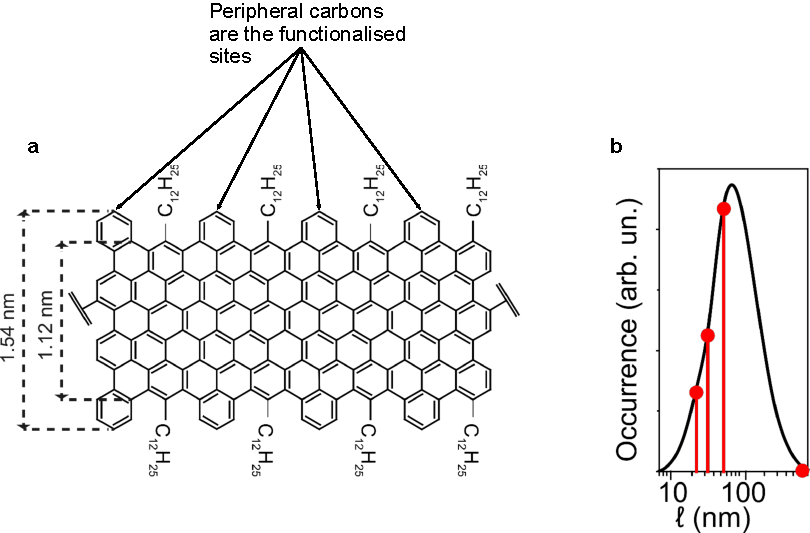
\includegraphics[width=\textwidth]{chapter_doping/figures/base_ribbon_length_distribution.pdf}
        \caption[Cove-4 GNR structure and Length Distribution]{\textbf{a,} Structure of a 4-Cove graphene nanoribbon. Highlighted are the carbon sites where dopant atoms are introduced through chemical synthesis. \textbf{b,} Distribution of MGNR lengths $l$ as obtained from size-exclusion chromatography on the polymerized molecular precursor (black). Red dots and vertical lines identify various length obtainable with different elution curves. Adapted from~\cite{dotti2018phd}.}
        \label{fig:chem_doping:base_ribbon_length_distribution}
    \end{center}
\end{figure}

Unfortunately these ribbon featured very poor solubility, even after several sonication and dilution cycles in most of the common organic solvents. Since it was not possible to carry out a thorough experimental study at the device level, we have investigated  the structural and electronic properties of GNR--H and compared them with the ones of GNR--OMe, GNR--Br, GNR--Cl, and GNR--Anthracene through DFT simulations.

\begin{figure}[hbtp]
    \begin{center}
        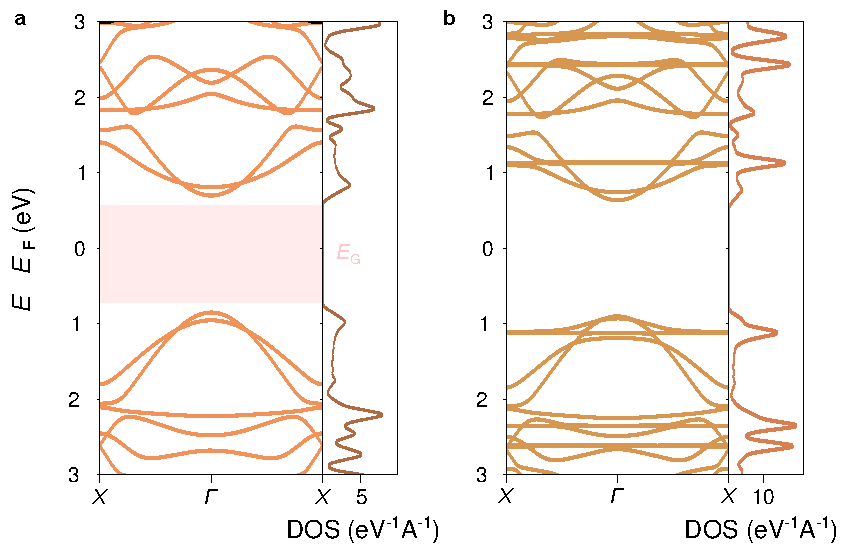
\includegraphics[width=\textwidth]{chapter_doping/figures/anthracene.pdf}
        \caption[DFT Band Structures and DOS of a 4-Cove GNR--H and a GNR--Anthracene]
        {\textbf{a,} Band structure and density of states for a 4-Cove GNR--H and \textbf{b,} a 4-Cove GNR--Anthracene calculated with the exchange--correlation functional GGA-PBE.}
        \label{fig:chem_doping:base_anthracene}
    \end{center}
\end{figure}

Ab-initio calculations were performed by using the \gls{LDA}-CA and the \gls{GGA}-PBE excahnge--correlation functionals as implemented in Siesta \cite{soler2002siesta, garcia2020siesta}. To simplify the geometry, alkyl chains were removed and replaced with hydrogen atoms. Sufficient vacuum distance is added along the non-periodic directions to avoid unwanted interactions. Numerical atomic pseudopotential was used together with an energy cut-off of 400 Ry. Monkhorst Pack k-point-grid was chosen to be ($20\times 1\times 1$) along the three Cartesian directions. The structure is optimized until the maximum force on the atoms is less than \SI{0.01}{\electronvolt\per\angstrom}.

\begin{figure}[hbtp]
    \begin{center}
        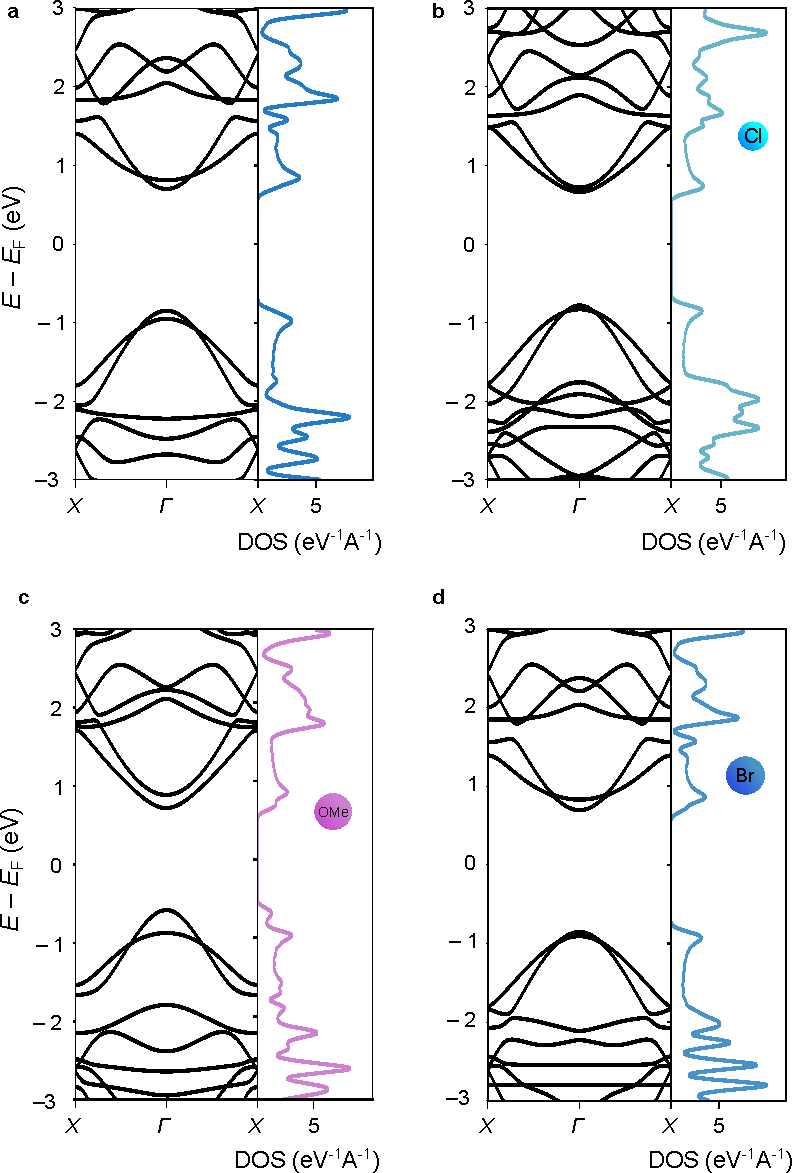
\includegraphics[width=\textwidth]{chapter_doping/figures/drawing.pdf}
        \caption[DFT Band Structures and DOS of Chemically-Functionalised MGNRs]
        {Band structure and density of states for graphene nanoribbons decorated with various electron donors or acceptors resulted after applying the GGA approximation for the exchange--correlation energy term.}
        \label{fig:bandstructure_chem_doping}
    \end{center}
\end{figure}

Fig.~\ref{fig:chem_doping:base_anthracene} shows the comparison between the base case and the same ribbon functionalised with anthracene along the edges. Compared to the base case, the introduction of anthracene groups introduces sharpe features in the \gls{DOS} in correspondence of flat lines in the band structure, which may are attributable to a more kind of discrete spectrum. This observation is in agreement with predictions at the \gls{NEGF} level and known as even--odd conductance effect~\cite{vcercnevivcs2020even}. In particular, for functional groups with an odd number of rings, the local density of states resides on the site of the guest molecule which is bound convalently to the nanoribbon, resulting in a non-negligible interaction between the continuum of states in \gls{GNR} and the localised state on the edge-attached adduct.

Furthermore, at this level of theory it appears that the when anthrance groups are introduced along the edges the particle-hole symmetry is broken, as the band structure  spectrum is no longer symmetric with respect to the Fermi energy



Fig.~\ref{fig:bandstructure_chem_doping} compares the band structures and \gls{DOS} between GNR-H (top-left) and other chemical dopants. In the case of GNR-OMe, four electron-donating methoxy groups per repeating unit have been considered, while six negative inductive Clorine groups were considered for GNR-Cl. Firstly, it is possible to observe the frontier bands in case of GNR-OMe are $\simeq\SI{0.5}{\electronvolt}$ higher than those of GNR-H, likely due to charge redistribution induced by the methoxy groups.

In addition to this, the DFT simulations suggests that the aromatic structure of GNR-OMe might be slightly distorted becuase of the steric repulsion introduced by the methoxy groups. In order to test this hypothesis, we performed a DFT simulation of a non-planar GNR-H having the same spatial distortion of GNR-OMe without the methoxy groups. The methoxy groups were replaced by hydrogen atoms after the geometric optimization of GNR-OMe, while keeping the distorted aromatic core fixed. The results suggests that the geometric distortions are responsible for only one-half of the bandgap shrinkage, i.e. \SI{125}{\milli\electronvolt}, while the other half can be ascribed to the larger effective width of the $\pi$-conjugated system of GNR-OMe due to the delocalization of the frontier states over the oxygen of the methoxy groups.

Interestingly, despite the fact that both the bromine and chlorine substitutions share electrons with the ribbon preferentially via $\sigma$-bond, GNR--Cl exhibits a more pronounced bandgap contraction (Tab.~\ref{tab:bandgaps}) and a decrease in effective mass $m^*$ at the $\Gamma$ point of the conduction band. The same holds true for the case of methoxy substitution. As the effective mobility $\mu_\textrm{eff}$ of charge carriers is proportional to the inverse of their effective mass, a decrease in the effective mass of the charge carriers may be advantageous for their transport, possibly resulting in better device performance. On the other hand, no appreciable deviation from the base case is observed for the ribbon functionalized with Br groups, which could be explained by a lower electronegativity and consequently a lower ability to induce charge rearrangement of the ribbon frontier orbitals.



% explain the doping shift from normal n for the Cl and Br to p for methoxy

\begin{table}
    \caption{\label{tab:bandgaps}
        Calculated bandgaps using different exchange--correlation implementations.}
    \[
        \begin{array}{lcccc}
            \hline\textit{Edge}        & \textrm{LDA}-\textrm{CA} & \textrm{GGA}-\textrm{PBE} & \Delta E_g \textrm{(CA)} & \Delta E_g \textrm{(PBE)}             \\
            \textit{functionalisation} & (\si{\electronvolt})     & (\si{\electronvolt})      & (\%)                     & (\%)                                  \\
            \hline
            \text{--H}                 & 1.57                     & 1.55                      & -                        & -                             \Tsmall \\
            \text{--Anthracene}        & 1.55                     & 1.54                      & -0.96                    & -0.77                                 \\
            \text{--Br}                & -                        & 1.55                      & -                        & -0.04                                 \\
            \text{--Cl}                & 1.45                     & 1.44                      & -7.62                    & -6.77                                 \\
            \text{--OMe}               & 1.31                     & 1.3                       & -16.21                   & -16.1                                 \\
            \text{--CH3}               & 1.56                     & 1.55                      & -0.44                    & -0.25                                 \\
            \text{--CN}                & 1.58                     & 1.56                      & +0.62                    & +0.74                                 \\
            \text{--NH2}               & 1.36                     & 1.35                      & -13.03                   & -12.9                                 \\
            \text{--COOH}              & 1.55                     & 1.53                      & -0.84                    & -0.98                                 \\
            \text{--NO2}               & 1.47                     & 1.47                      & -6                       & -5.24                                 \\
            \text{--OH}                & 1.47                     & 1.46                      & -5.82                    & -5.82                                 \\
            \hline
        \end{array}
    \]
\end{table}

\section{Methoxy-Edge-Decorated MGNR-Based Field-Effect Transistors}\label{ch:doping:sec:methoxy}

In order to test the idea of chemically-induced doping, we fabricated two kinds of \glspl{FET} using GNR--H (base case) and GNR--OMe (methoxy). As reported in Tab.~\ref{tab:bandgaps}, methoxy groups are predicted to induced the largest relative change in the bandgap compared to the base case, and the

GNR--OMe were provided by Dr Alicia G{\"o}tz and prof.\ Akimitsu Narita from the Okinawa Institute of Science and Technology. The ribbons have a structure similar to the one reported in Fig.~\ref{fig:chem_doping:base_ribbon_length_distribution}a, where the peripheral carbons are functionalised with methoxy functional groups. The Hammett equation classifies a methoxy substituent in the para position as an electron-donating group on a benzene ring, but as an electron-withdrawing group in the meta position~\cite{anslyn2006modern}. The methyl free rotation is expected to induce a considerable change in the Hammett prediction becuase of the steric effect, leading to a change in the ortho position reactivity, which otherwise follows the same trend as the para position~\cite{gotz2022band}.

\begin{figure}[hbtp]
    \begin{center}
        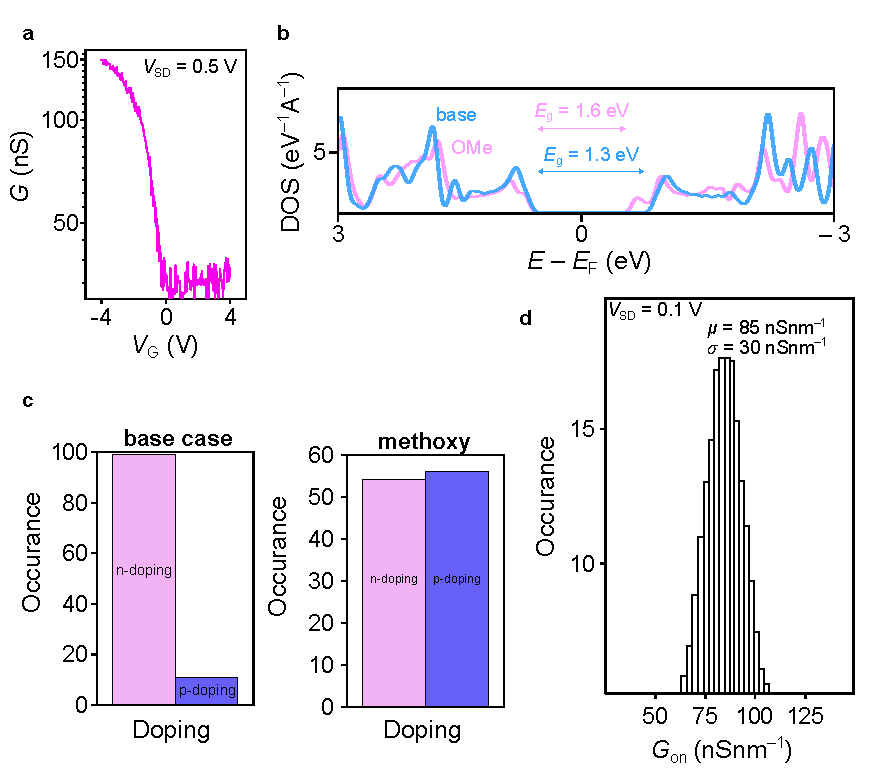
\includegraphics[width=\textwidth]{chapter_doping/figures/methoxy_fet_stat_1.pdf}
        \caption[Methoxy-Functionalised GNRFETs]
        {
            \textbf{a,} Typical transfer $G$--$V_\textrm{G}$ curve of a p-type methoxy-functionalised \gls{GNRFET} with $\SI{0.5}{\volt}$ of biase applied.
            \textbf{b,} Calculated electron states density at \gls{DFT}--PBE level for GNR--H (base case) and GNR--OMe.
            \textbf{c,} Compared to the base case, when methoxy decorations are introduced there is a significant increase in the number \glspl{GNRFET} displaying p-type doping.
            \textbf{d,} Histogram for the on-state conductance normalised by the channel width $W_\textrm{ch}$.
        }
        \label{fig:methoxy_fet_stat_1}
    \end{center}
\end{figure}

\Glspl{GNRFET} were fabricated as detailed in Ch.~\ref{ch:fabrication}. Fig.~\ref{fig:methoxy_fet_stat_1}a shows a typical transfer characteristics curve with $I_\textrm{on}/I_\textrm{off}\simeq 10^1$, that is about three order of magnitude below digital application requirements~\cite{schwierz2013graphene}. Numerical \gls{DFT} calculations using the PBE pseudopotential suggest that the bandgap could shrink by a $\simeq 16\%$ (Fig.~\ref{fig:methoxy_fet_stat_1}b) when four electron-donating methoxy groups per repeating unit are attached to the \gls{GNR}. Because we are not including any many-body corrections~\cite{onida2002electronic}, this estimate is likely to be an overestimate of the true value. After several discussions with our collaborators we concluded that quantifying the amount of functionalisations is challenging because the polymerization technique used to introduce the chemical groups is not stereospecific~\cite{gotz2022band}.

In an attempt to quantify the effctiveness of the chemical functionalization, we measured the position of the charge neutrality point (CNP), which reflects the charge doping level in graphene, for hundreds of devices (Fig.~\ref{fig:methoxy_fet_stat_1}c). For the base case, \glspl{GNRFET} display almost exclusively n-type of doping (CNP at negative voltages), which confirms the observation of a larger bandgap for hydrogen-terminated \gls{GNR}~\cite{liu2011chemical}. On the other hand, methoxy groups increase significantly the number of devices with p-type doping. We advanced two explanations for this experimental observation. First, as we can see from Fig.~\ref{fig:methoxy_fet_stat_1}b the valence band is more affected than the bottom of the conduction band, since it is upshifted compared to the base (blue) case. This effect has also been reported when \gls{GNR} edges are decorated with electron-withdrawing groups~\cite{carbonell2017doping, ohtomo2018interpolymer}. Furthermore the methoxy groups could introduce holes but also p-type impurities in the transistor channel~\cite{schedin2007detection, jung2009charge}.

We evaluated performance metrics after the introduction of the methoxy groups, namely the on-state conductance $G_\textrm{on}$ (Fig.~\ref{fig:methoxy_fet_stat_1}d) and the subthreshold swing $SS$ (Fig.~\ref{fig:methoxy_SS_slope}).
Because surface techniques like as \gls{AFM} could not be used, we estimated the number of graphene nanoribbons in the conduction channel as follows. Since graphene nanogaps produced through electroburning are $d\simeq\SI{5}{\nano\metre}$, and the ribbons width is $w_\textrm{GNR}=\SI{1.12}{\nano\metre}$ (Fig.~\ref{fig:chem_doping:base_ribbon_length_distribution}) we estimate that the channel width $W_\textrm{ch}$ contains about 5 nanoribbons, thus $W_\textrm{ch}\simeq\SI{5}{\unit{GNR\per\nano\metre}}$. This number is supported also by similar estimates from Monte Carlo and STM~\cite{llinas2017short,lin2022scaling, de2016substrate}. The on-state conductance $G_\textrm{on} = G_\textrm{sat}/(w_\textrm{GNR}W_\textrm{ch})=\SI{0.03}{\siemens\per\milli\metre}$ and conductivity $\sigma=Gl_\textrm{GNR}/w_\textrm{GNR}=\SI{1.4}{\micro\siemens}$ is orders of magnitude lower compared to values from carbon nanotubes ($\sim\SI{500}{\micro\ampere\per\micro\metre}$), excluding for this ribbon wiring applications.



To quantify the concentrations of chemically-induced charge carries control over the number of functional groups along is necessary, but unfortunately our colleagues could not achieved it yet. Furthermore, one interesting hypothesis to test would be to check if there is an edge-selectivity of the process, for example by adding chemical decorations on ribbons of varying width, and look for a width-dependent response: intuitively, narrower ribbons should yield an increased response, being the number of edge sites relative to ribbon basal plane sites higher.

\begin{figure}[hbtp]
    \begin{center}
        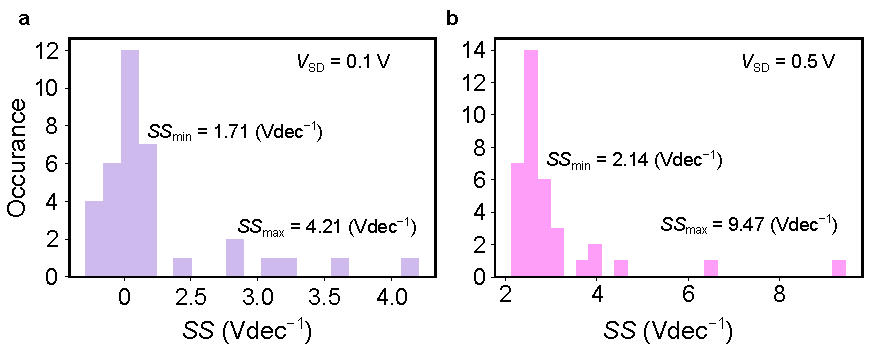
\includegraphics[width=\textwidth]{chapter_doping/figures/methoxy_SS_slope.pdf}
        \caption[Switching Behaviour of Methoxy-Functionalised GNRFETs]
        {
            \textbf{a,} Switching histograms at low ($V_\textrm{SD}=\SI{0.1}{\volt}$) and \textbf{b,} medium ($V_\textrm{SD}=\SI{0.5}{\volt}$) drain voltages in ambient conditions.
        }
        \label{fig:methoxy_SS_slope}
    \end{center}
\end{figure}

At room temperature, we see no fast switching behaviour (Fig.~\ref{fig:methoxy_SS_slope}). The experimental values we measured are at least three orders of magnitude lower than the most competitive \glspl{CNTFET} (Tab.~\ref{intro:tab:cnt_devices} in Ch.~\ref{ch:introduction}). The poor control over the conductive channel degrades as the drain voltage is increased (Fig.~\ref{fig:methoxy_SS_slope}b) which is typical of a tranistor's response. This could possibly due to the higher concentration of holes injected through the methoxy groups~\cite{tokunaga1991substrate}.

We would want to point out, however, that the conductive channel in our devices is poorly defined, as we do not have exact control over the structural arrangement of the nanoribbons on top of the leads due to dropcasting. The addition of 3D bulky groups that suppress the $\pi$--$\pi$ interactions between individual ribbons (see also Ch.~\ref{ch:solubility}) might further increase the performance of transistors like these. Future research should compare the device performance of GNR--OME with and without maleimide groups.



\section{Substitutional Doping Through Heteroatoms Embedding in Graphene Nanoribbons Lattice}\label{gnr-hybrid:sec:measure}

The idea of using chemical functionalisations to induce a preferential doping in carbon nanostructures is not new.
Several proposals have indeed demonstrated the possibility to tune the conductance of ropes~\cite{bockrath2000chemical} and individual~\cite{zhou2000modulated, ewels2005nitrogen} carbon nanotubes by introducing dopants
in the walled structure, thus leading to p--n junctions and Esaki diodes. These procedures, however, tend to be uncontrolled leaving the substrate with unknown number of dopants per carriers.

In contrast, bottom-up chemical synthesis may provide a viable route to structurally well-defined graphene ribbons with uniform structures in which the dopants are introduced along the edges through control of the chemical functionalisations. Amonngst the various ribbon edges, cove GNRs have attracted a lot of interest for several reasons. First of all, their synthesis can be completely achieved in solution without any surface-assisted methodolgy. Secondly, the steric tension induced by the lateral groups on the structure makes them typically non-planar, open up possibility to investigate not only optical properties but also spin--orbit coupling effects in carbon nanostructures, which have remained so far elusive from experimental evidence.

\begin{figure}[hbtp]
    \begin{center}
        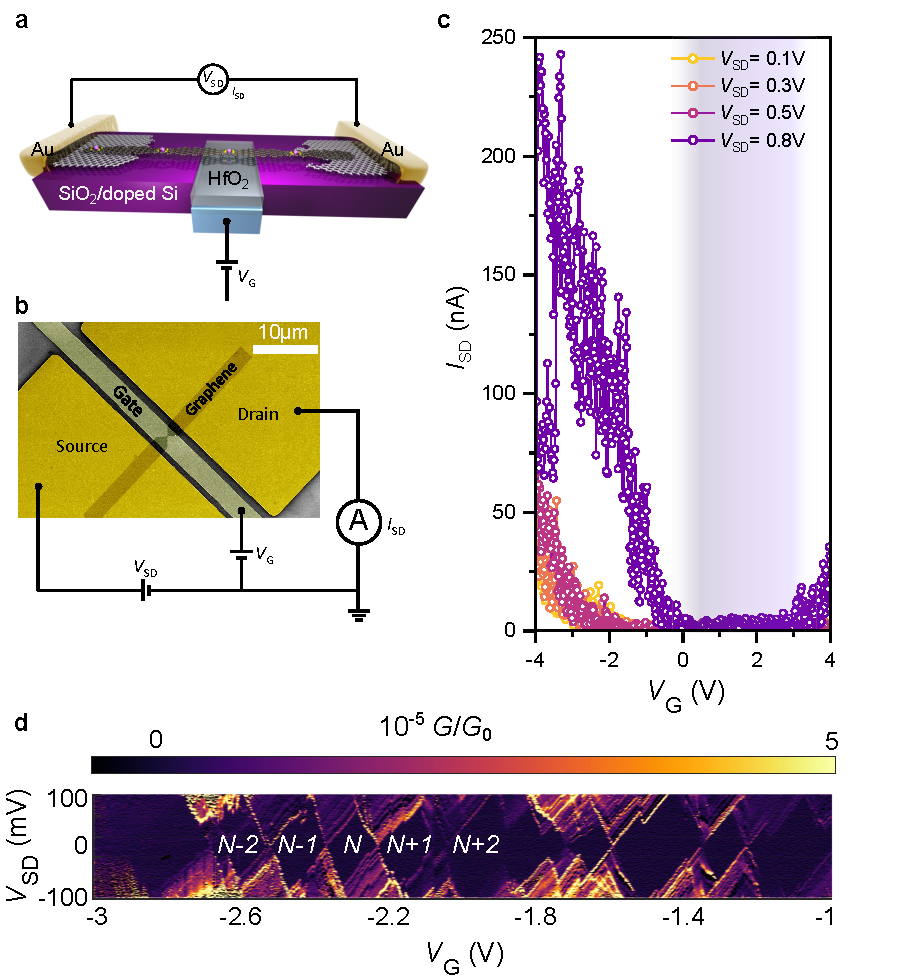
\includegraphics[width=\textwidth]{chapter_doping/figures/gnr-hybrid_cartoon_sem_fet_set.pdf}
        \caption[GNR-porphyrin Hybrid Device: Low- and Room-Temperature Comparison]
        {
            \textbf{a,} Cartoon of the device schematic and the electrical wiring.
            \textbf{b,} False-scale SEM image of a device sample, hihglighting the Au pads, \ce{HfO2} gate, graphene leads, and the electrical connections for biasing the device.
            \textbf{c,} Room-temperature \gls{FET} response of a device under different biases. The device present a bandgap in the positive region of $V_\textrm{G}$, demonstrating p-doping effect. The estimated $E_g\simeq\SI{2}{\electronvolt}$ is in line with what we expect from optical absorption measurements.
            \textbf{d,} Clear demonstration of \gls{SET} behaviour for \gls{pGNR} when these objects are cooled down at cryogenic ($T=\SI{20}{\milli\kelvin}$) temperatures. The possibility of discriminating n-doping from p-doping at RT makes the mapping of the various charge states more easy.
        }
        \label{fig:gnr-hybrid_cartoon_sem_fet}
    \end{center}
\end{figure}

Furthermore, theoretical calculations have shown that the wave functions for the frontier crystal orbitals are fully delocalized across the ribbon width, in contrast to zigzag-GNRs (with localized states at the ribbon edges), with electronic band gap of cove-edged GNR infinite ribbon settling around 1.70 eV, and mobilities values in the order of thousands \si{\cm\square\per\V\per\second} for both electrons and holes~\cite{Liu2015}.

\co{First Paragraph: Device Fabrication}
Feedback-controlled electroburning is used to produce nanogaps, localised at the bowtie constriction, with widths between \SIrange{1}{10}{\nano\metre}. $I_\textrm{SD}-V_\textrm{SD}$ characteristics are recorded for all devices immediately after nanogap formation and after drop-casting approximately \SI{8}{\micro\litre} suspension of the \gls{pGNR} hybrids.

Suspensions were prepared by sonicating a dry powder of the \glspl{pGNR} in toluene (\SI{0.02}{\milli\gram\per\milli\litre}) for \SI{60}{\minute}. Several cycles of the electroburning protocol were performed, up to three different gate voltages for each device, and each time scanning in gate voltage at fixed bias to check for residual graphene quantum dots.

If any are found, the electroburning process is restarted at that gate voltage to clear the residual graphene. For all devices, the resistance limit was set at \SI{2.3}{\giga\ohm}. Devices which show an increase in current post-deposition are selected for wire bonding and further measurements. Transport measurements were performed in an Oxford Instruments Triton 200 dilution refrigerator using low noise DC electronics. All measurements were performed at a temperature of 20 mK. Differential conductance is retrieved by numerical differentiation of the measured current.

\co{Second Paragraph: Device 1 Results}
The full charge-stability diagram of a typical device cooled down to \SI{25}{\milli\kelvin} is shown in Fig.~\ref{fig:gnr-hybrid_cartoon_sem_fet}d. Yellow colours indicate regions of higher differential conductance while darker colours indicate lower regions of differential conductance. At gate voltages below \SI{-1}{\volt} clear signs of Coulomb blockade diamonds are present. Outside this gate voltage range, the level of current is close to the noise limit of the current-to-voltage converter used in our transport setup. In the absence of a discernible repeating pattern, it is possible that the faint diamonds visible at higher gate voltages are caused by spurious charges injected possibly through the gate oxide or surface states.

\begin{table}
    \caption{\label{tab:gnr-hybrid_peaks_fitting}
        Lorentzian fit parameters extracted by fitting a low-bias gate trace. The two peaks are separated by 600 meV in voltage, which could be assigned to the single-electron charge transition $N \leftrightarrow N+1$, where $N$ is the number of electrons on the ribbons which is unknown. Reported errors are fitting errors.}
    \[
        \begin{array}{ccc}
            \hline\textrm{Peak Position}  & \textrm{Lifetime Broadening} & G_\textrm{max}                   \\
            \textrm{(\si{\electronvolt})} & (\si{\milli\electronvolt})   & (G_0)                            \\
            \hline
            -1.64                         & 2.5\pm0.2                    & (4.5\pm0.2)\times10^{-7} \Tsmall \\
            -1.04                         & 2.8\pm0.2                    & (2.8\pm0.1)\times10^{-7}         \\
            \hline
        \end{array}
    \]
\end{table}

From Fig.~\ref{fig:gnr-hybrid_sd_eadd} we can read the addition energies for the different charge states by reading the height of each diamond, within the assumption that only one electron is exchanged for each charge transition. Across all the diamonds, we can extract the gate coupling which measures the effectiveness of the gate voltage to change the chemical potential of the ribbon. We found $\alpha_\textrm{G}\simeq\SI{0.65}{\electronvolt\per\volt}$ averaged across all the measurable charge states, with a slight asymmetric coupling with the drain lead for this particular device.

Furthermore, two peaks at $V_\textrm{G}\simeq\SI{-2.5}{\volt}$ and $V_\textrm{G}\simeq\SI{-1.5}{\volt}$ are closed, so we can extract their lifetime broadening by fitting a low-bias ($V_\textrm{SD}\simeq\SI{2.6}{\milli\volt}$) gate trace with a Breit--Wigner resonance (Tab.~\ref{tab:gnr-hybrid_peaks_fitting}). The tunneling couplings with the graphene leads are one order of magnitude stronger than the majority of tunneling coupling reported for devices fabricated with normal graphene nanoribbons.

\begin{figure}[hbtp]
    \begin{center}
        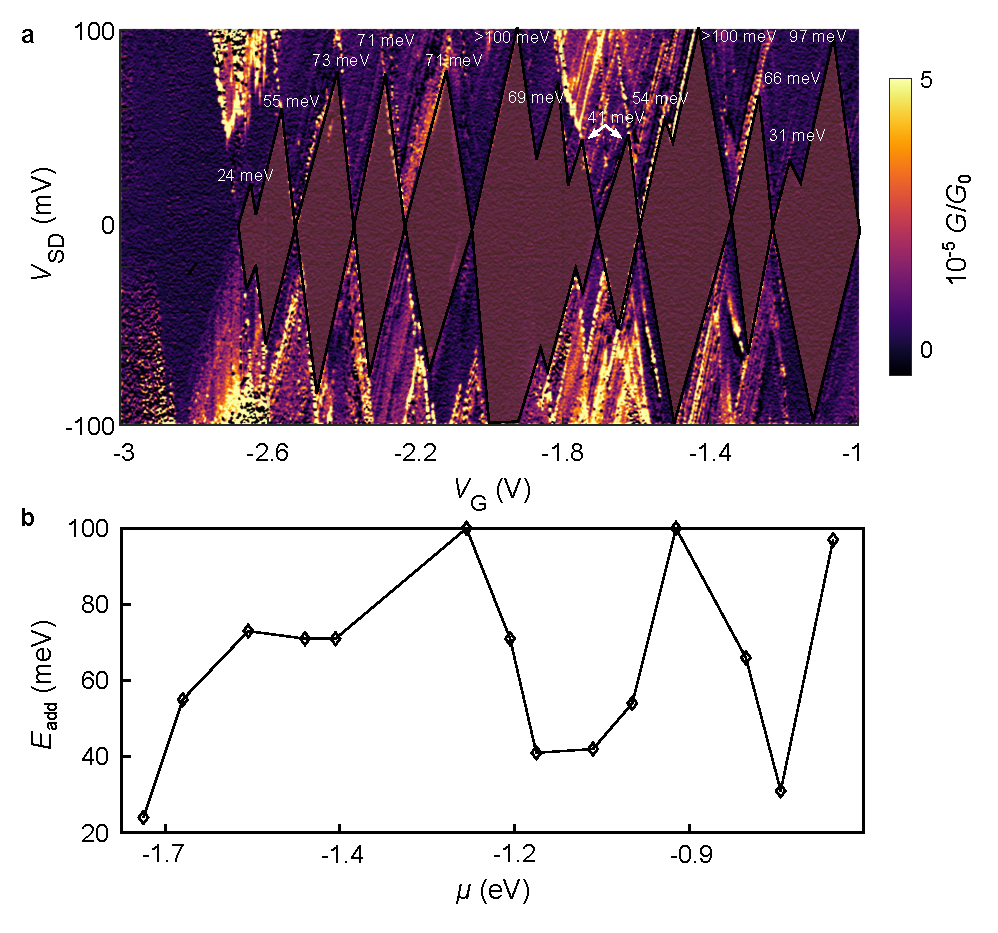
\includegraphics[width=\textwidth]{chapter_doping/figures/gnr-hybrid_sd_eadd.pdf}
        \caption[GNR-Hybrid Stability Diagram and Addition Energies]
        {\textbf{a,} Low-temperature stability map demonstrating Coulomb blockade and well-defined charge states. \textbf{b,} We extract the addition energies from the diamond height and plot them as a function of the chemical potential felt by the ribbon as a result of the application of a gate voltage, assuming a constant gate coupling of $\alpha_\textrm{G}\simeq\SI{0.65}{\electronvolt\per\volt}$ for all charge states.}
        \label{fig:gnr-hybrid_sd_eadd}
    \end{center}
\end{figure}



\co{Third Paragraph: Determination of pGNR Length}

A possible explanation for the observed values for the tunneling coupling might be the different length of the \gls{pGNR} compared to the bottom-up ribbons studied in in the last two chapters. Since the thickness of the \ce{HfO2} oxide on top of the gate is approximately \SI{10}{\nano\metre}, we had to experimentally measure the capacitance of the the oxide in order to extract a more accurate value.

A parameter needed to determine the length of \glspl{pGNR} is the relative permittivity of the gate oxide. Because of the ultra-thin nature of the oxide used in these devices, it is not possible to rely on the bulk value for \ce{HfO2} and it must be experimentally determined~\cite{robertson2004high}.
This was achieved by microfabricating capacitors on the devices using the following approach. A chip is selected from the same wafer used to fabricate devices 1, 2 and 3. The substrate is \ce{O2}-plasma etched to remove the \gls{CVD} graphene layer and prepare the surface for lithography (20 minutes, 25 sccm and 100 percent power). An array of top electrodes is patterned using electron-beam lithography, metal deposition and lift-off. The design consists of overlapping top electrode of varying areas with the gate contact pad separated by the ALD-deposited HfO2 dielectric layer as shown in Figure 7. A small region is removed from the top electrode allowing a W probe to make contact through the oxide and electrically contact the bottom electrode.

An Andeen--Hagerling 2550A ultra-precision capacitance bridge is used to measure the capacitance between the top electrode and the bottom-gate electrode. The measurement is carried out at room temperature in a probe station. The stray capacitance of the probe station and experimental wiring is measured and is found to be insignificant when compared to the values obtained from the microfabricated capacitors. The excitation voltage applied by the bridge is limited to \SI{1}{\volt} RMS to reduce the risk of dielectric breakdown. $\varepsilon_r$ is thus determined by:

\begin{equation}
    \varepsilon_r = \frac{Cd}{\varepsilon_0 A},
\end{equation}

where $d = \SI{10}{\nano\metre}$ is the oxide thickness, $\varepsilon_0$ is the permittivity of free space, and $A$ is overlapping area of the top and bottom electrode measured using microscopy. The obtained values are shown in Table 1. An average value of $\varepsilon_r = 15.41$ is used in all length calculations.

\begin{table}
    \caption{\label{tab:measured_capacitance}
        Measured values of electrode area, capacitance and $\varepsilon_r$  for several capacitors. These are consistent across various randomly selected points onto a single chip. Errors for $\varepsilon_r$ were found to be at the third decimal place.}
    \[
        \begin{array}{cccc}
            \hline\textrm{Device} & \textrm{Electrode Area}     & \textrm{Measured Capacitance} & \varepsilon_r        \\
            \textrm{name}         & (\si{\micro\metre\squared}) & (\si{\pico\farad})            &                      \\
            \hline
            \textrm{A}1           & 7455                        & 101.1\pm1.0                   & 15.3\pm0.02  \Tsmall \\
            \textrm{A}2           & 4542                        & 62.4\pm0.6                    & 15.51\pm0.02         \\
            \textrm{C}3           & 2402                        & 32.5\pm0.3                    & 15.26\pm0.02         \\
            \textrm{E}1           & 7438                        & 100.6\pm1.0                   & 15.3\pm0.02          \\
            \textrm{I}1           & 7433                        & 103.3\pm1.0                   & 15.7\pm0.02          \\
            \hline
        \end{array}
    \]
\end{table}

Since the distance between the ribbon and the gate is comparable to the ribbon width we would need to employ the general formula for retrieving the length from the charging energy~\cite{shylau2009capacitance}, i.e.
\begin{equation}
    l = \frac{e^2\left(8 d \arctan{\frac{w}{4 d}}+w \log {1+\frac{16 d^2}{w^2}}\right)}{4\pi E_C \epsilon_r \epsilon_0}
\end{equation}
%
By using this formula, we estimate lengths for the sample we have measured of about \SI{25}{\nano\metre} for $E_C\simeq\SI{40}{\milli\electronvolt}$.

\co{Middle Part: FET Behaviour}

This section presents several devices with \gls{FET} characteristics. All measurements were taken in ambient conditions with a semi-automated, 3-probe system Cascade Microtech Summit 12000 as described in Ch.~\ref{ch:fabrication}. \ce{CuBe} probes with tip diameters of \SI{30}{\micro\metre} were used to contact the source and drain \ce{Au} pads, while \ce{W} probes with tip diameters of \SI{10}{\micro\metre} were used for the gate probe. Figure 8 shows an example of a device a we obtained.

The device exhibits p-type doping and the on-state channel conductance $G$ normalised by the width of the \gls{GNR} ($w_\textrm{GNR} = \SI{1.2}{\nano\metre}$) increases from \SI{0.05}{\siemens\per\milli\metre} at $V_\textrm{SD} = \SI{0.1}{\volt}$ to \SI{0.1}{\siemens\per\milli\metre} when $V_\textrm{SD}$ is increased to \SI{0.5}{\volt}; the on-state conductivity $\sigma = GL/w_\textrm{GNR} = \SI{3.73}{\micro\siemens}$ for a channel length $L\simeq\SI{40}{\nano\metre}$ (the length of the channel is estimated by averaging the transport data of multiple devices at low temperature).

The device was switched off when the gate voltage $V_\textrm{G}$ was larger than \SI{0.5}{\volt} and had good $I\textrm{on}/\textrm{off}\simeq 10^3$ as the source--drain voltage was set to \SI{0.1}{\volt}. Off-state conductance was estimated around $G_\textrm{off}\simeq\SI{6}{\pico\siemens\per\nano\metre}$ at $V_\textrm{SD}=\SI{0.1}{\volt}$ and increasing as the $V_\textrm{SD}$ was increased, despite exhibiting consistent switching behaviour of about $SS\simeq\SI{400}{\milli\volt}$~dec$^{-1}$ and indicating good gate control over the conduction channel.

On top of that, almost no hysteresis was measured under ambient conditions. The hydrophobic nature of the sandwich established by the ribbon and graphene leads considerably minimises the undesired hysteresis in the transfer characteristics of the transistors, which is caused by the presence of water close to the GNR--dielectric contact (gate-voltage sweep rate was \SI{44}{\milli\volt\per\second}), and outperforming early carbon nanotube FET~\cite{weitz2007high}.

\begin{figure}[hbtp]
    \begin{center}
        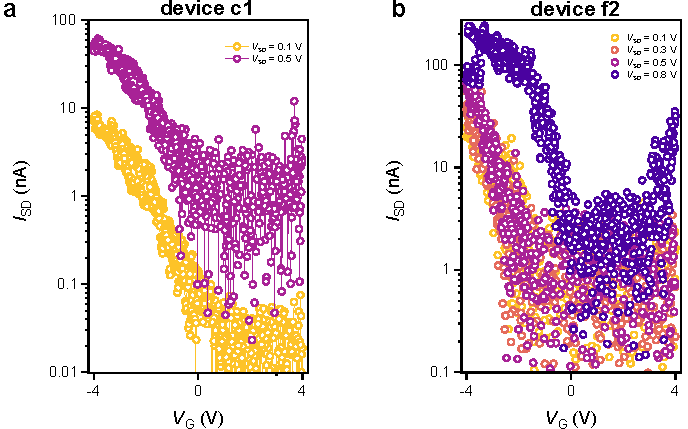
\includegraphics[width=\textwidth]{chapter_doping/figures/gnr-hybrid_FET_c1_f2.pdf}
        \caption[GNR-Hybrid Field-Effect Transistors at Room Temperature]
        {\textbf{a,} Semi-log plot of the transfer curves for a p-type \gls{FET} device obtained with \gls{pGNR} acquired at low and medium biases. \textbf{b,} Another p-type device with the transfer curves acquired under equispaced $V_\textrm{SD}$ voltages.}
        \label{fig:gnr-hybrid_FET_c1_f2}
    \end{center}
\end{figure}

While the on-state current is not directly related to the bandgap energy $E_g$, the off-state current strongly depends on $E_g$~\cite{kim2011role}. Assuming the synthesised \gls{pGNR} is an intrinsic semiconductor and its band structure has a mid-gap alignment with the source--drain contacts, the smallest (off-state) current will occur when both the conduction and valence bands are flat. If transport is controlled by thermal carrier emission, the on--off ratio will depend exponentially on the temperature. It is then possible to give an estimate of $E_g$ for a devices, which in case of device c1 is

\begin{equation}
    2k_BT\log{\qty{\frac{I_\textrm{on}}{I_\textrm{off}}}=E_g\simeq\SI{327}{\milli\electronvolt}},
    \label{eq:on_off_ratio_bandgap}
\end{equation}

Since it is typically difficult to establish the threshold voltage in transfer characteristics without ambiguity, conventional \glspl{FET} are frequently compared using the so-called field-effect mobility. This is device-specific rather than material-specific, and includes effects such as contact resistances and surface effects~\cite{durkop2004extraordinary}. We have estimated both the linear and the saturation \gls{FET} mobilities for several devices.

The conduction channel is pinched off when $V_\textrm{SD} = V_\textrm{G} - V_\textrm{Th}$, where $V_\textrm{Th}$ is the threshold voltage at which the device switches on. In this condition, the current cannot increase substantially anymore and saturates to a value $I_\textrm{SD,sat}$ identifiable as a plateau by either plotting the semi-logarithmic plot of  transfer characteristics or by simply visualising the output characteristics. If channel-shortening effects caused by the depletion region at the drain are neglected, the saturation current can be obtained by substituting $V_\textrm{SD}$ with $V_\textrm{G} - V_\textrm{Th}$, and within the gradual-channel approximation the drain–saturation current may be written as~\cite{zaumseil2007electron}

\begin{equation}
    I_\textrm{SD,sat} = \frac{w_\textrm{GNR}}{2L}\mu_\textrm{sat}C_\textrm{G}(V_\textrm{G}-V_\textrm{Th})^2,
\end{equation}
%
where $C_\textrm{G}$ is the gate capacitance per unit area. From the capacitance measurements detailed above we extract a $C_\textrm{G}=\SI{1.4e-2}{\farad\per\metre\squared}$. We estimate a saturation mobility (also called field-effect mobility) for this particular device to be \SI{0.8}{\centi\metre\squared\per\volt\per\second}. We further estimate the field-effect mobility in the linear regime ($V_\textrm{G}\gg V_\textrm{SD}$) by extracting the gradient of $I_\textrm{SD}$ versus $V_\textrm{G}$ at constant $V_\textrm{SD}=\SI{0.1}{\volt}$

\begin{equation}
    \mu_\textrm{lin} = \pdv{I_\textrm{SD}}{V_\textrm{G}}\frac{L}{w_\textrm{GNR}C_\textrm{G}V_\textrm{SD}}=\frac{g_mL^2}{C_\textrm{GS}V_\textrm{SD}}.
\end{equation}

We remark that the capacitance values $C_\textrm{G}$ and $C_\textrm{GS}$: the former represents the capacitance between the nanoribbon segment that spans across the gate and the gate itself. Therefore, we have estimated that the capacitance per unit area for a ribbon of $L\simeq\SI{40}{\nano\metre}$ and $w_\textrm{GNR}=\SI{1.2}{\nano\metre}$ placed on top of a gate of thickness $d\simeq\SI{10}{\nano\metre}$ is

\begin{equation}
    C_\textrm{GS} = \frac{\varepsilon_0\varepsilon_rA}{d}=\SI{0.7}{\atto\farad},
\end{equation}
%
For device c1 we estimate a linear \gls{FET} mobility $\mu_\textrm{lin}\simeq\SI{4}{\centi\metre\squared\per\volt\per\second}$.

Device f2 in Fig.~\ref{fig:gnr-hybrid_FET_c1_f2} reproduces qualitatively a similar behaviour. In comparison with device c1, this device exhibits $I_\textrm{on}/I_\textrm{off}\simeq 10^2$, which then would correspond to a $E_g\simeq\SI{220}{\milli\electronvolt}$ by using Eq.~\ref{eq:on_off_ratio_bandgap}. The peculiarity of this device is that a current saturation limit is reached only at $V_\textrm{SD}=\SI{0.8}{\volt}$, with a $\Delta V_\textrm{gap}\simeq\SI{3}{\volt}$, and the off-state current tends to increase with increasing bias. The gate has good control ($SS\simeq\SI{400}{\milli\volt}$~dec$^{-1}$) over the conductive channel at small biases, and excellent control $SS\simeq\SI{160}{\milli\volt}$~dec$^{-1}$ at $V_\textrm{SD}=\SI{0.8}{\volt}$, which is amongst the highest values measured across our devices. Furthermore, the on-state channel conductance $G$ normalised by the channel width reaches values as high as \SI{0.2}{\siemens\per\milli\metre} and on-state conductivity $\sigma\simeq\SI{6}{\micro\siemens}$. We report slightly higher values for the mobility of this device as we extracted $\mu_\textrm{sat}=\SI{3.5}{\centi\metre\squared\per\volt\per\second}$ and $\mu_\textrm{lin}=\SI{16}{\centi\metre\squared\per\volt\per\second}$.

In Table 3, we present the linear and saturation mobilities for a variety of devices. Since our pGNR has molecularly defined edges, we explain these values by assuming that the effective mobility decreases as the ribbon width approaches sub-5 nm. The linear-mobility values correlate well with those expected by theoretical estimation~\cite{geng2017graphene}, but the saturation-mobility values have not yet been found. At room temperature, the effective mobilities are predicted to be limited by acoustic phonons. Nonetheless, if the surface-impurity density is large, this may become the major scattering mechanism, and values in the range of \SIrange{10}{1000}{\centi\metre\squared\per\volt\per\second} are expected~\cite{fang2008mobility}, which is consistent with the values we measured.

\begin{table}
    \caption{\label{tab:extracted_mobilities}
        Linear and saturation mobilities extracted from the transfer characteristics of several devices.}
    \[
        \begin{array}{ccc}
            \hline \text { Device } & \mu_{\operatorname{lin}}                        & \mu_{\text{sat}}                                      \\
            \textrm{name}           & (\si{\centi\metre\squared\per\volt\per\second}) & (\si{\centi\metre\squared\per\volt\per\second})       \\
            \hline \text { E5 }     & 5                                               & 1                                             \Tsmall \\
            \text { C1 }            & 4                                               & 0.8                                                   \\
            \text { F2 }            & 16                                              & 3.5                                                   \\
            \text { C6 }            & 39                                              & 4                                                     \\
            \text { C4 }            & 11                                              & 4.3                                                   \\
            \hline
        \end{array}
    \]
\end{table}


\section{Outlook and Perspectives}\label{gnr-hybrid:sec:summary}

The role of chemical-induced doping in \glspl{GNRFET} is still an open problem. We have seen in Sec.~\ref{ch:doping:sec:methoxy} that methoxy functionalisations could be responsible in the doping observed through the shift of the CNP. Unfortunately, the shift of the CNP is a controversial debate, and often contaminations have produced the same effect. Furthermore, we could not test other graphene nanoribbons with different functionals groups. Two next steps would then be necessary for elucidating if there is a real doping effect at the device level. Firstly, groups subtracting electron density from the nanoribbons should be used. Following discussion with our collaborators it appears that this task is not easy to solve as attaching n-type of functionalisations are extremely challenging becuase of the lower edge reactivity to Diels--Alder polimerization reactions. Secondly, our measurements should be repeated in vacuum. in fact, repeated measurements in air have demonstrated to naturally p-doped graphene substrates.

Since the attachment along the edges of n-type dopants seems within the reach we have demonstrated in Sec.~\ref{gnr-hybrid:sec:measure} that a viable alternatiuv
As we have seen in


\section{Summary}
\Glspl{pGNR} were provided by Dr Qiang Chen and prof.\ Harry Anderson. Fanmiao Kong assisted me in configuring the electronic computations on the ARC supercomputing centre, which we thank for its cooperation and assistance in troubleshooting issues when jobs were not running.